\documentclass[12pt]{article}

\usepackage{amsmath}
\usepackage{graphicx}
\usepackage[margin=1in]{geometry}
\usepackage[style=authoryear,backend=biber]{biblatex}
\addbibresource{impact.bib}

\begin{document}
\title{Foreign Buyer Revisionism}

\section{Introduction}

Taxes and restrictions on foreign purchases of residences have been implemented
in multiple jurisdictions worldwide with the stated purpose of making homes
more affordable for domestic residents. For example, in extending a ban on
foreign purchases of Canadian residential real estate, a government press
release stated: ``For years, foreign money has been coming into Canada to buy
up residential real estate, increasing housing affordability concerns in cities
across the country, and particularly in major urban centres. Foreign ownership
has also fueled worries about Canadians being priced out of housing markets in
cities and towns across the country.''\footnote{\textcite{gOC}.}

There are theoretical and empirical reasons to expect foreign buyer taxes to
succeed in bringing down local housing prices, many of which are detailed in a
comprehensive study by \textcite{favilukisVanNieuwerburgh}. The disincentive to
purchase homes should reduce the number of buyers considering purchasing
properties and lower willigness to pay among remaining foreign buyers. This
reduction in prices hurts landlords and incumbent property owners through lost
property value and rents, but makes home ownership more affordable for locals
who do not yet own homes. There may be an associated loss of construction jobs,
and the analysis in \textcite{favilukisVanNieuwerburgh} does not consider the
effect of reciprocal taxes on domestic residents who may wish to purchase
property overseas.\footnote{It is not obvious that a target country would wish
	to reciprocate to disincentivize the host country's tax. For example,
	China, the source of most foreign buying in Canada prior to the recent
spate of taxes (per, e.g. \textcite{ctvNews}) has made efforts to discourage capital
flight.}

Existing studies of the impact of the entry and exit of foreign buyers on local home prices
present estimated effects that range from modest to quite large, as summarized
in \textcite{davidoffZheng}. \textcite{LiShenZhang},
\textcite{gorbackGlobalCapitalLocal2020}, \textcite{pavlovImmigrationFlows},
and \textcite{BadarinzaRamadorai} find that within metropolitan areas,
submarkets exposed to foreign buyers see larger price increases when the types
of foreign buyers prone to buy in those submarkets face increased incentives to
buy overseas. \textcite{DachisDurantonTurner}, \textcite{klevenBest},
\textcite{kopczukMunroe}, and \textcite{davidoffLeigh} find, as a general
matter, that increasing transaction taxes on housing purchases leads to fewer
transactions and lower prices. \textcite{HartleyForeign},
\textcite{andalfattoEstimatingEffectMetro2023}, \textcite{DuYinZhang}, and
\textcite{pavlovForeignBuyerTaxes} collectively find that foreign buyer taxes
in Australia, Canada, and New Zealand led to lower prices.

As \textcite{favilukisVanNieuwerburgh} observe, foreign buyers may not leave
homes empty, but rather rent them out to locals. In their calibration, this
changes the social welfare effect of foreign buyers from negative to slightly
positive. The effect of out of town buyers is moderate because local investors
are highly price sensitive in their demand for rental properties, and out-of-town
buyers represent a small share of overall capital investment. In this way,
foreign buyers represent a slightly positive form of capital accumulation. This
is a salient consideration, as British Columbia has imposed significant taxes on empty
homes and vacation properties in urban areas while also imposing significant
taxes on foreign buyers, and the Canadian federal government has both imposed
taxes on empty homes owned by foreigners and has temporarily banned the
purchase of single residences by foreigners.

At the time of writing, the market for condominiums in Vancouver and Toronto
are so weak that construction has stopped. While indicative of falling prices,
the lack of condo presales has led some observers to suggest that the taxation
of foreign buyers has overshot, leading to a negative supply response larger
than the positive demand response on prices from foreign buying, such that
locals have been adversely affected. It is thus worthwhile asking whether there
is empirical evidence supporting the idea that foreign buyers, particularly in
the presence of empty homes taxes, may have positive welfare effects and their
taxation adverse effects on housing affordability for locals. QUOTE GOODMAND AND RENNIE HERE

There are several channels through which foreign buyers could have positive
affordability effects. First, per \textcite{favilukisVanNieuwerburgh}, foreign
buyers may rent houses to locals, particularly in the presence of an empty
homes tax.\footnote{This observation is echoed in the BC context in a policy
brief, \textcite{Goodman}.} Second, foreign buyers may purchase condominiums in
the presale phase of condominium development and then assign their contracts
prior to completion. The presence of foreign presale purchasers would raise
presale prices, encouraging the supply of condominiums, but with no increase in
demand for occupied space. The net effect of that form of investment should be
positive for affordability for end users, with an adverse competition effect
for locals who wish to occupy homes purchased through the presale channel.

A third way in which foreign buyers could have a beneficial effect on
housing affordability for local apartment buyers if they have a relative
preference for quality, and if there is a high degree of vertical
differentiation within buildings. In that case, foreign buyers could make
projects more profitable than they would otherwise be, increasing supply, but
without crowding out local demand. This would be a variant of the positive
``pecuniary externality''

In the next sections, we review some available economic evidence on the extent to which 
the channels alluded to above are operative in the Vancouver housing market.

\section{A simple framework for evaluating foreign buyer effects on local housing afforadbility}

As discussed above, foreign buyers may or may not compete for the same units as
locals, and may rent the homes they own to locals. A simple model provides a
way to organize data to evaluate likely affordability effects of taxes and
quantity restrictions on foreign buyers.

Suppose that there is a very large number of potential foreign buyers with
infinitely elastic demand for housing units at a price of $p_{f}$, assumed
always higher than the equilibrium willingness to pay among locals that comes
from the demand curve $q_{l}\left(p_{l}\right)$. The fraction of buyers that
are foreign $\alpha$ in each building is then determined by a government
policy, here assumed to be exogenously
chosen.\footnote{\textcite{FavilukisVanNieuwerburgh} allow foreign demand to be
affected by the local price and by an time-varying exogenous factor.}

Developers charge different prices to foreign and local buyers. This could
arise through two channels. First, foreign buyers might demand higher quality
units, e.g. penthouses for which they have a much greater willingness to pay
than locals, but have relatively little interest in lower-floor, ordinary
units. Second, developers might market a fraction of presale units 
overseas, and the law of one price might not force equality of pricing if
foreign buyers are constrained in their ability to participate in ordinary
presale or resale markets.\footnote{An allegedly common practice, see, e.g.
\texttt{https://vancouver.citynews.ca/2017/06/06/developer-intend-give-overseas-buyers-first-shot-vancouver-project/}.}

The supply of housing units is given by a function $q_{s}\left(\bar{p}\right)$,
increasing in price. $\bar{p}$ is the average price at which homes are sold,
$\bar{p} \equiv \left[1-\alpha\right]p_{l} + \alpha p_{f}$.

Some fraction of housing units purchased by foreign buyers are rented out to
locals, and some presale buyers flip their homes prior to occupancy of
buildings. Call $z$ the fraction of units owned by foreign buyers that are
unavailable to locals. The magnitude of $z$ might be taken as a measure of how
important affordable home ownership is, beyond prioritizing renters. A large
$z$ value could thus indicate that local consumers renting from foreigners is
seen as undesirable by policymakers, whereas $z=0$ might indicate that
converting owner units to rental is not undesirable.\footnote{Indeed,
policymakers have implemented a range of policies designed to convert homes
from owner-occupied to rental, such as favorable financing from crown
corporation CMHC for rental housing and local zoning policies that allow more
density for purpose-built rental apartments than for condominium buildings.}

Equating supply and demand for local buyers yields the following equation:

\begin{equation}
	\label{eq:localSD}
	\left[1-\alpha z\right]q_{s}\left(\left[1-\alpha\right]p_{l} + \alpha p_{f}\right) = q_{l}(p_{l}).
\end{equation}

Developers will supply more units the higher the average price per unit paid by locals and foreign buyers weighted by their share of all units built. Implicitly differentiation of equation \eqref{eq:localSD} indicates that the effect on local prices of a small increase in the foreign buyer share depends is:

\begin{equation}
	\label{eq:implicit}
	\frac{dp_{l}}{d\alpha} = -\frac{-zq_{s} + \left[1-\alpha z\right]q_{s}'\left[p_{f}-p_{l}\right]}{\left[1-\alpha z\right]\left[1-\alpha\right]q_{s}'-q_{l}'}.
\end{equation}

The denominator of the right hand side of equation \eqref{eq:implicit} is positive as long as supply slopes up and local demand slopes down in price. The numerator of the right hand side of equation \eqref{eq:implicit} is negative, so that price falls with an increase in the permitted foreign share, if:

\begin{equation}
	\label{eq:sign}
	\text{sign}\left(\frac{dp_{l}}{d\alpha}\right) = \text{sign}\left(1-\underbrace{\frac{q_{s}'p_{l}}{q_{s}}}_{\text{supply elasticity}}\times\underbrace{\frac{p_{f}-p_{l}}{\bar{p}}}_{\text{foreign price premium}}\times\underbrace{\frac{1-\alpha z}{z}}_{\text{Domestic occupancy intensity}}\right).
\end{equation}

Summarizing the analysis, allowing a little more foreign buying will improve affordability when:

\begin{itemize}
	\item The supply of homes is highly responsive to prices.
	\item Foreign buyers pay much more than locals for apartments in the same buildings.
	\item Most units in new buildings are occupied by locals in a way that government appreciates, i.e. there are few foreigner owners ($\alpha$ is low), or foreign owners commonly rent to locals and that arrangement is not viewed as objectionable.
\end{itemize}

\section{Some evidence on the determinants of foreign buyer affordability effects}

\subsection{Supply elasticity}

Out-of-town buyers (somewhat different definitionally from buyers subject to foreign buyer taxes) seem to have been concentrated in housing markets with relatively inelastic supply. \textcite{paixao2021housing} provides a list of Canadian CMAs by housing supply elasticity (estimated from one-year differences in prices and quantities), and Figure \ref{fig:elasticityNonResident} plots that elasticity against non-resident ownership. 

The modest supply elasticities in markets like Toronto and Vancouver (where supply elasticity is low and out-of-town demand relatively high) suggest that foreign ownership may have adverse afforability consequences if not paired with limits on empty homes. It is worth remarking, though, that non-resident ownership was modest in all large Canadian CMAs as of 2018.

\begin{figure}
	\centering
	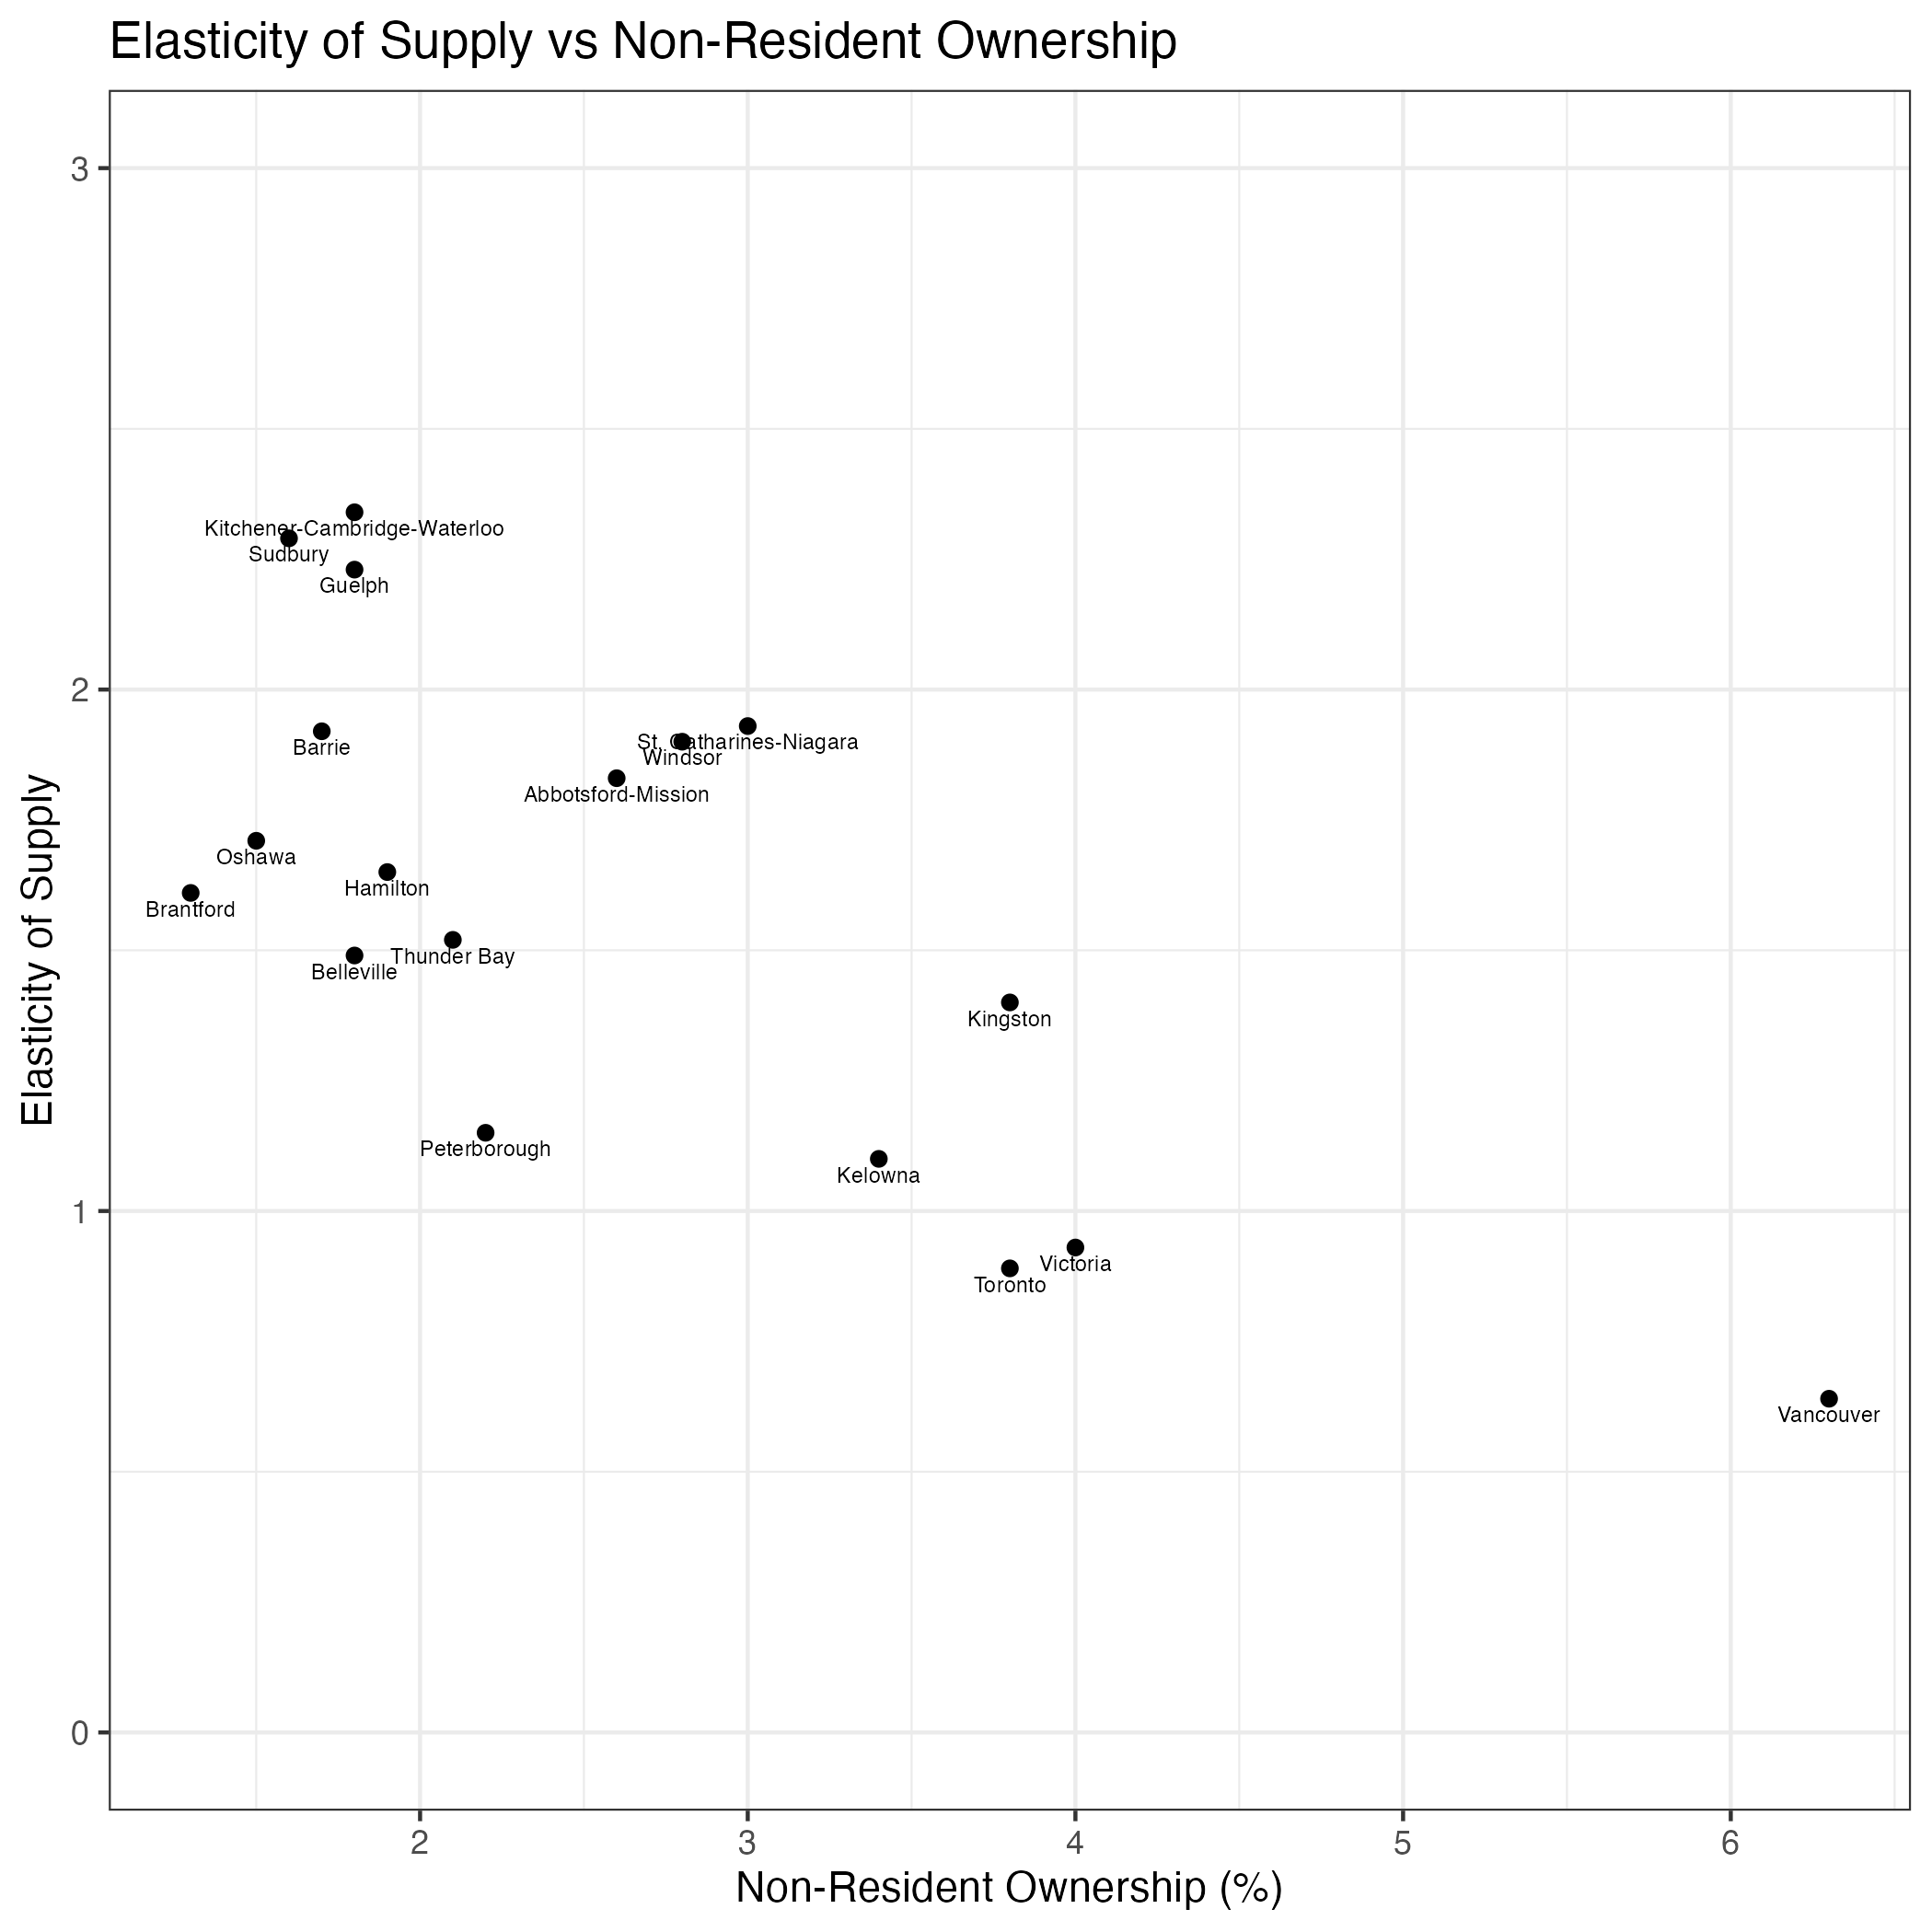
\includegraphics[width=0.8\textwidth]{"~/OneDrive - UBC/foreignImpact/text/elasticityOwnership.png"}
\caption{\label{fig:elasticityNonResident} Non-resident ownership and housing supply elasticity in Canadian CMAs. Sources: \textcite{paixao2021housing} and CHSP table ``Residency participation of residential properties, by property type and period of construction'' for 2018 estimates. (charted values of elasticities merged on CMA names by ChatGPT).}
\end{figure}

\subsection{Do foreign buyers pay more for units in the same building?}

Equation \eqref{eq:sign} suggests that foreign buyers can have a positive supply effect when the units in which they stimulate supply are largely occupied by locals (where $\alpha z$ is close to zero). If foreign buyers pay higher prices than local primarily because they occupy different buildings than locals, it is not easy to see a positive supply effect for locals.\footnote{\textcite{FavilukisVanNieuwerburgh} account for the job creation effects of the supply effect when foreign buyers purchase homes.}

Foreign buyers might pay more than locals for units in the same building either
by facing different prices for the same units, or by specializing in
particularly luxurious units within buildings. We cannot observe whether the
law of one price is violated, e.g.  through differential presale pricing
overseas.

There is some scope for answering the question of whether foreign buyers purchase higher quality units within
buildings than local buyers with available data, at least for the resale
market, if not for the critical presale market. Figure
\ref{fig:variance_decomposition} uses data taken from condominium resales in
Greater Vancouver between 2010 and 2023, provided by BC Assessment.
The plot measures the year of transactions on the horizontal axis. On the
vertical axis are measures of the variance of the natural logarithm of
transaction prices by year. The red line plots the variance of all transaction
prices. The green plots the variance of mean prices across
buildings.\footnote{If there were only one transaction for each building with a
transaction in a given year, the red and green lines would coincide.} The blue
line plots the mean variance of log transaction prices within buildings. 

The dashed vertical line in Figure \ref{fig:variance_decomposition} coincides
with the imposition of the foreign buyer tax in July, 2016. Consistent with
foreign buyers demanding more expensive units (as non-resident buyers do in the
CHSP data),\footnote{See also  the overall variance of prices drops sharply in the years after the
tax, consistent with loss of an important luxury segment of the market.
However, the reduction in price variance appears to be almost entirely driven
by

\begin{figure}
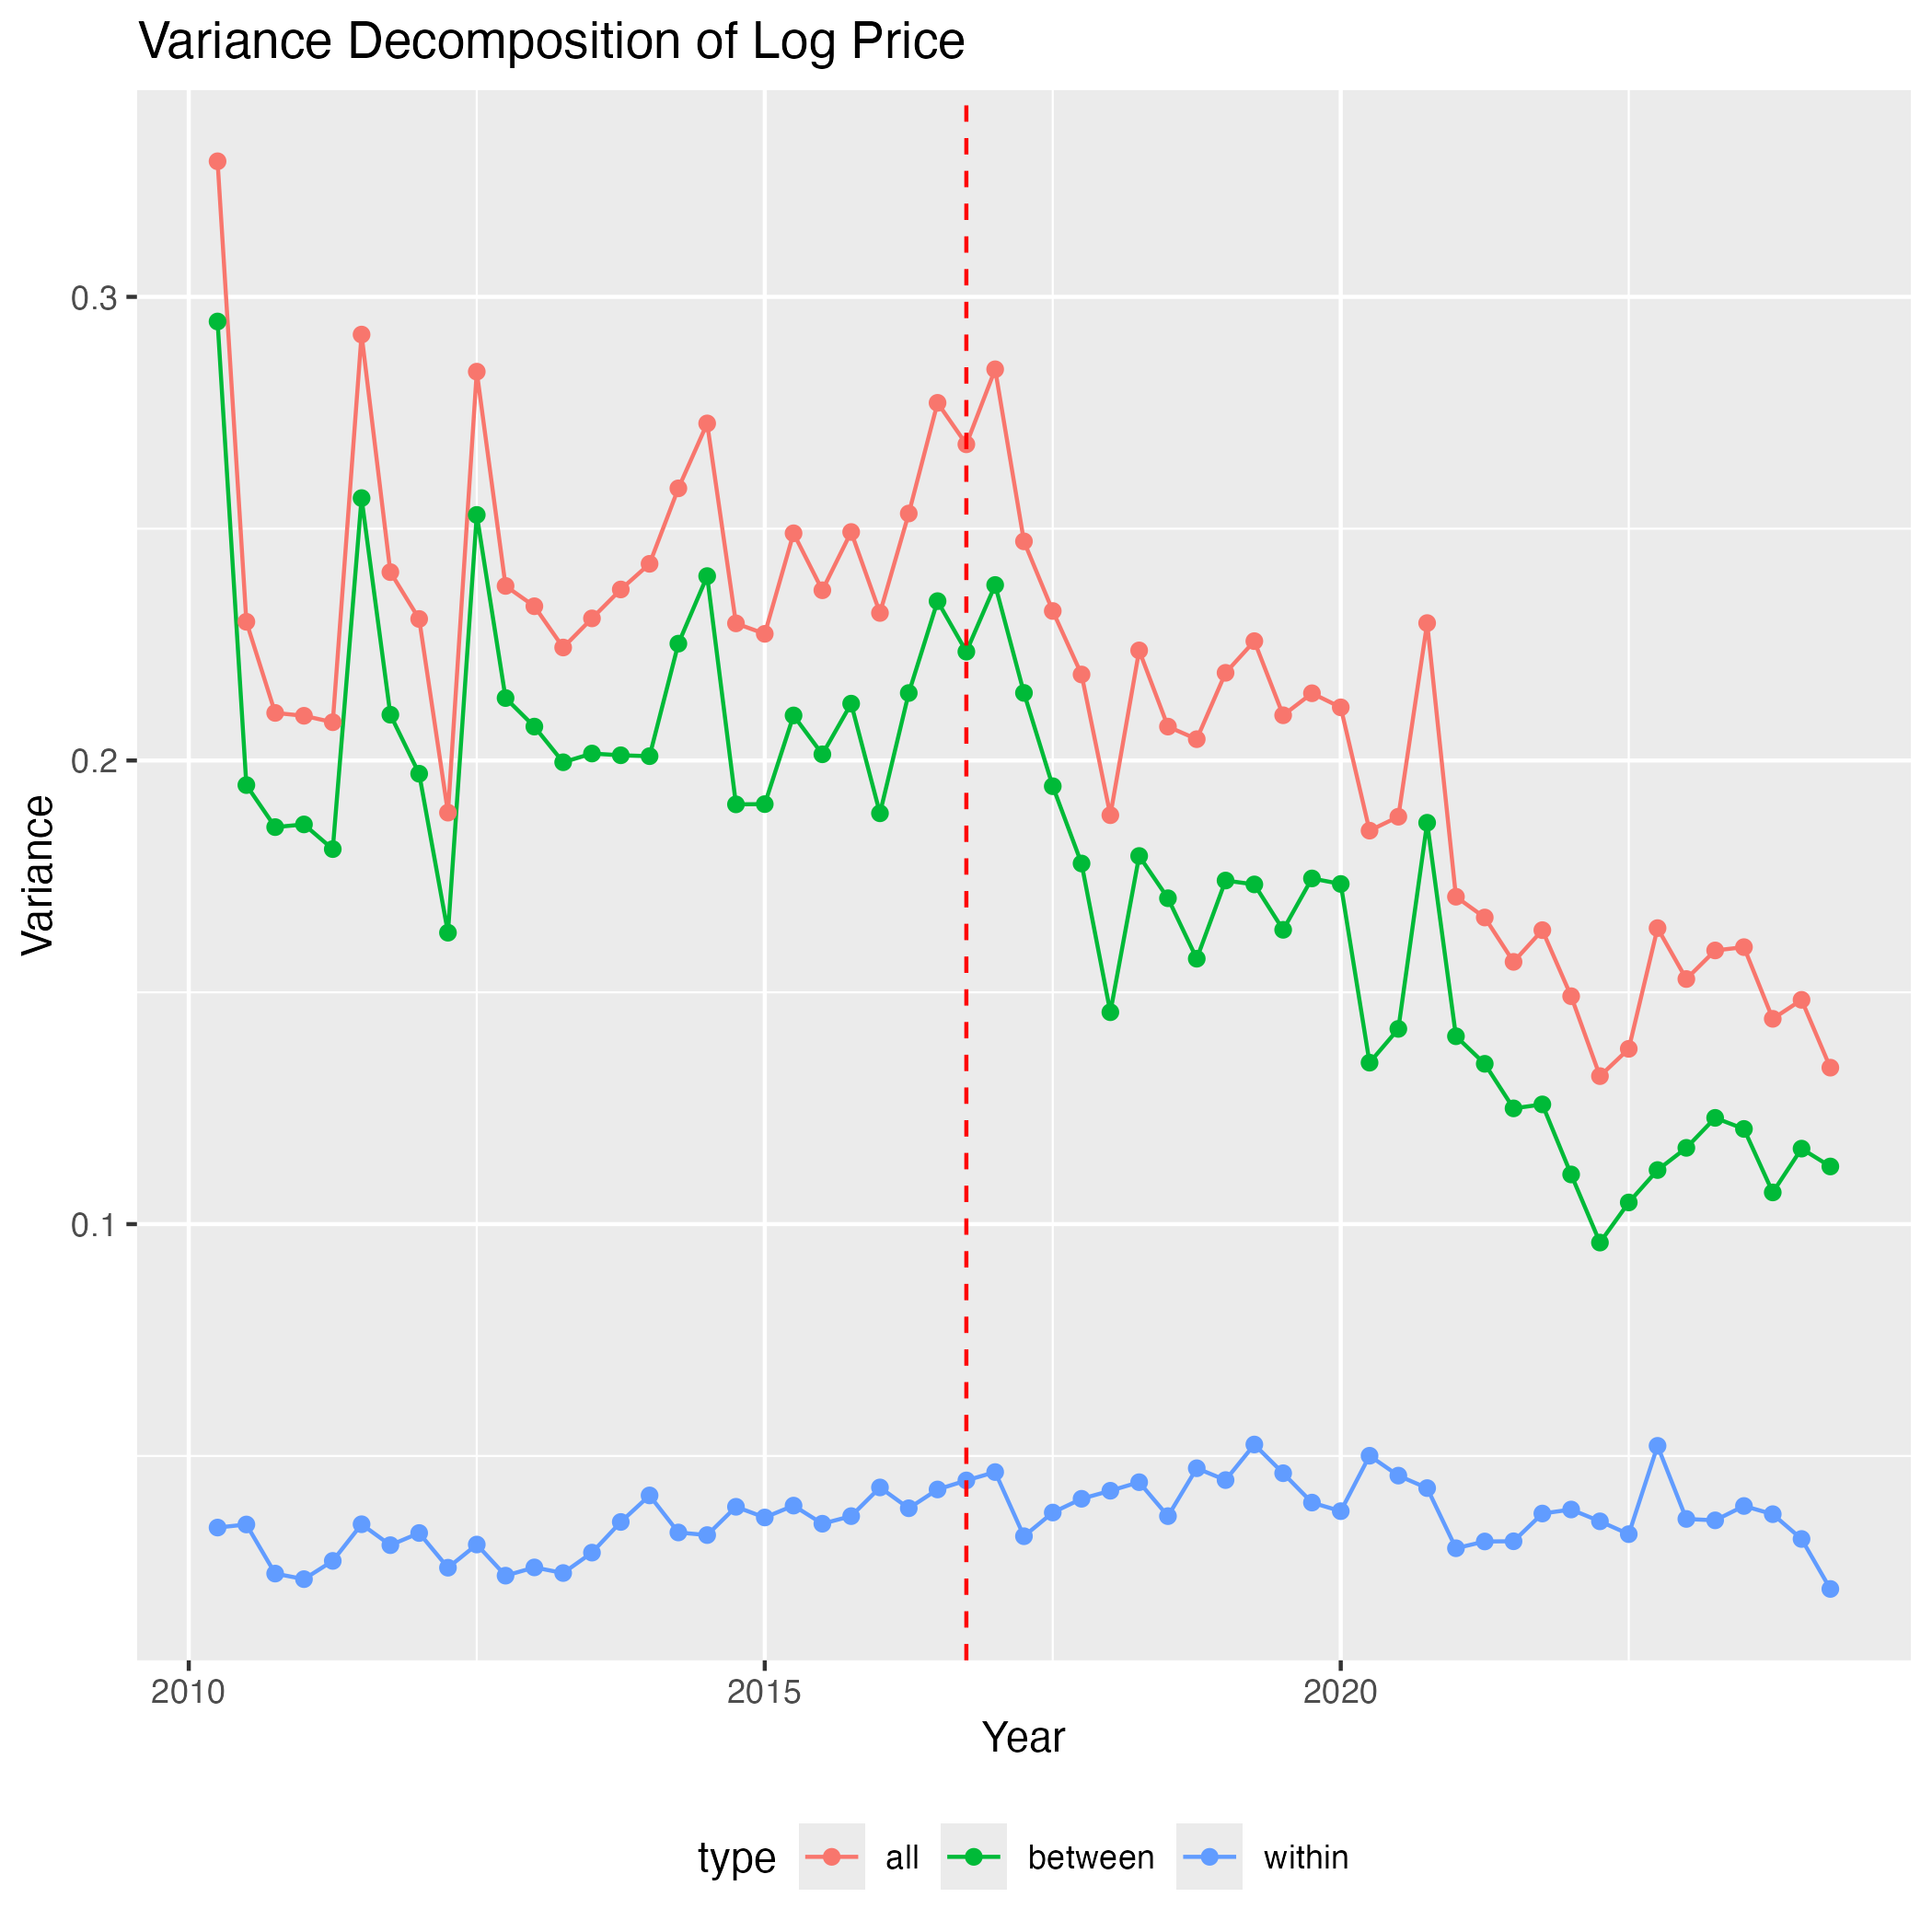
\includegraphics[width=\textwidth]{"~/OneDrive - UBC/foreignImpact/text/variance_decomposition.png"}
\end{figure}


\section{Stock and flow of foreign purchases in Greater Vancouver}

For the years starting in 2018, the Canadian Housing Statistics Program has used its access to ownership data on the universe of Canadian residences to publish statistics on ownership by residency status in Canada. This is an approximation of foreign ownership, because some owners who live overseas are Canadian citizens or permanent residents, and hence exempt from foreign buyer taxes. Also, some Canadian residents are not yet landed immigrants, and hence are subject to the foreign buyer tax. Thus CHSP represents an approximation of the stock of ``foreign'' ownership over time. Unfortunately, the stock measure is not readily available prior to 2018. Between 2018 and 2022, the number of non-resident owners in the Vancouver Census Metropolitan Area grew from 24,135 to 26,350, but fell from 9.6\% to 9.0\%.

The apparent declining stock of foreign ownership as a share of all residences
is matched by a declining share of the flow into ownership. The B.C. provincial
government started collecting data on the nationality of residential property
buyers shortly before implementing the additional property transfer tax of 15\%
on foreign buyers in mid-2016. In the month (July) prior to implementation,
15\% of purchases in Metro Vancouver involved foreign participation. For the
years since, the fractions have been as shown in Table \ref{tab:fbt}. COVID and
the national foreign buyer ban have likely contributed to the decline over time
in foreign participation.

\begin{table}
	\caption{\label{tab:fbt} Fraction of residential transactions in Metro Vancouver with foreign participation, per BC Property Transfer Tax data. Source: \texttt{https://catalogue.data.gov.bc.ca}}
	\begin{tabular}{ll}
		\hline
		Year & Fraction of transactions with foreign participation \\
		\hline\hline
		2017 & 3.7\% \\
		2018 & 2.9\% \\
		2019 & 2.0\%\\
		2020 & 1.4\%\\
		2021 & 1.1\%\\
		2022 & 1.3\%\\
		2023 & 0.9\%\\
		2024 & 0.9\%\\
		\hline
	\end{tabular}
\end{table}

\section{Do foreign buyers leave homes empty?}

Depending on whether empty homes taxes are set at a sufficiently high level or not, foreign buyer taxes may be desirable if foreign owners both (a) tend to leave homes empty for much of the year, rather than occupying them full time or renting them out to locals, and (b) are not responsive to taxes in that behaviour. 

In the presence of the B.C. empty homes tax regime, foreign owners who retain their
properties most commonly rent them out. Per \textcite{specTax2019}, of 3,709
foreign owners deemed subject to the empty homes tax in 2018, a large majority no
longer held empty homes in 2019. 1,205 of these foreign owners subject to the
Speculation and Vacancy tax transitioned to renting their homes out in 2019,
1,413 sold their property, 951 remained subject to the tax, and 66 transitioned
to using the home as a primary residence. 

\subsection{Presale flips}

Another politically unpopular group of housing investors ... that is British Columbia has implemented an additional tax on profits from capital gains on homes held for less than two years. That tax applies also to flipping presale contracts



\end{document}
